% IoU definition figure (TikZ).
% Coordinates in drawio-style px (1 unit = 0.02 cm, y pointing down). Requires tikz.
% Usage: \resizebox{<width>}{!}{% IoU definition figure (TikZ).
% Coordinates in drawio-style px (1 unit = 0.02 cm, y pointing down). Requires tikz.
% Usage: \resizebox{<width>}{!}{% IoU definition figure (TikZ).
% Coordinates in drawio-style px (1 unit = 0.02 cm, y pointing down). Requires tikz.
% Usage: \resizebox{<width>}{!}{% IoU definition figure (TikZ).
% Coordinates in drawio-style px (1 unit = 0.02 cm, y pointing down). Requires tikz.
% Usage: \resizebox{<width>}{!}{\input{../figures/pipeline/iou_def.tex}}
% overlay/remember picture are reset so the figure keeps its size when placed
% inside an overlay tikzpicture node.
\begin{tikzpicture}[
    overlay=false, remember picture=false,
    x=0.02cm, y=-0.02cm,
    font=\fontsize{7}{8.5}\linespread{1}\selectfont\sffamily\bfseries,
    edge/.style={line width=1.1pt},
    key/.style={anchor=west, inner sep=0pt},
  ]
  \definecolor{iouGT}{HTML}{00FF00}
  \definecolor{iouPred}{HTML}{FF0000}
  \definecolor{iouInter}{HTML}{0000FF}
  \definecolor{iouUnion}{HTML}{E6E6E6}
  \definecolor{iouUnionKey}{HTML}{CCCCCC}
  \definecolor{iouUnionText}{HTML}{999999}

  % Union
  \fill[iouUnion] (320,40) rectangle (400,120);
  \fill[iouUnion] (340,60) rectangle (420,140);

  % Intersection hatch
  \begin{scope}
    \clip (340,60) rectangle (400,120);
    \foreach \d in {-60,-40,...,60}
      \draw[iouInter, line width=0.5pt] (340+\d,60) -- (400+\d,120);
  \end{scope}

  % Boxes
  \draw[edge, iouPred] (340,60) rectangle (420,140);
  \draw[edge, iouGT]   (320,40) rectangle (400,120);

  % Legend
  \draw[edge, iouGT]   (440,45) rectangle (450,55);
  \draw[edge, iouPred] (440,65) rectangle (450,75);
  \draw[iouInter, line width=0.6pt] (440,90) -- (450,90);
  \fill[iouUnionKey]   (440,105) rectangle (450,115);
  \node[key, text=iouGT]        at (462,50)  {GT};
  \node[key, text=iouPred]      at (462,70)  {Pred};
  \node[key, text=iouInter]     at (462,90)  {Intersection};
  \node[key, text=iouUnionText] at (462,110) {Union};
\end{tikzpicture}
}
% overlay/remember picture are reset so the figure keeps its size when placed
% inside an overlay tikzpicture node.
\begin{tikzpicture}[
    overlay=false, remember picture=false,
    x=0.02cm, y=-0.02cm,
    font=\fontsize{7}{8.5}\linespread{1}\selectfont\sffamily\bfseries,
    edge/.style={line width=1.1pt},
    key/.style={anchor=west, inner sep=0pt},
  ]
  \definecolor{iouGT}{HTML}{00FF00}
  \definecolor{iouPred}{HTML}{FF0000}
  \definecolor{iouInter}{HTML}{0000FF}
  \definecolor{iouUnion}{HTML}{E6E6E6}
  \definecolor{iouUnionKey}{HTML}{CCCCCC}
  \definecolor{iouUnionText}{HTML}{999999}

  % Union
  \fill[iouUnion] (320,40) rectangle (400,120);
  \fill[iouUnion] (340,60) rectangle (420,140);

  % Intersection hatch
  \begin{scope}
    \clip (340,60) rectangle (400,120);
    \foreach \d in {-60,-40,...,60}
      \draw[iouInter, line width=0.5pt] (340+\d,60) -- (400+\d,120);
  \end{scope}

  % Boxes
  \draw[edge, iouPred] (340,60) rectangle (420,140);
  \draw[edge, iouGT]   (320,40) rectangle (400,120);

  % Legend
  \draw[edge, iouGT]   (440,45) rectangle (450,55);
  \draw[edge, iouPred] (440,65) rectangle (450,75);
  \draw[iouInter, line width=0.6pt] (440,90) -- (450,90);
  \fill[iouUnionKey]   (440,105) rectangle (450,115);
  \node[key, text=iouGT]        at (462,50)  {GT};
  \node[key, text=iouPred]      at (462,70)  {Pred};
  \node[key, text=iouInter]     at (462,90)  {Intersection};
  \node[key, text=iouUnionText] at (462,110) {Union};
\end{tikzpicture}
}
% overlay/remember picture are reset so the figure keeps its size when placed
% inside an overlay tikzpicture node.
\begin{tikzpicture}[
    overlay=false, remember picture=false,
    x=0.02cm, y=-0.02cm,
    font=\fontsize{7}{8.5}\linespread{1}\selectfont\sffamily\bfseries,
    edge/.style={line width=1.1pt},
    key/.style={anchor=west, inner sep=0pt},
  ]
  \definecolor{iouGT}{HTML}{00FF00}
  \definecolor{iouPred}{HTML}{FF0000}
  \definecolor{iouInter}{HTML}{0000FF}
  \definecolor{iouUnion}{HTML}{E6E6E6}
  \definecolor{iouUnionKey}{HTML}{CCCCCC}
  \definecolor{iouUnionText}{HTML}{999999}

  % Union
  \fill[iouUnion] (320,40) rectangle (400,120);
  \fill[iouUnion] (340,60) rectangle (420,140);

  % Intersection hatch
  \begin{scope}
    \clip (340,60) rectangle (400,120);
    \foreach \d in {-60,-40,...,60}
      \draw[iouInter, line width=0.5pt] (340+\d,60) -- (400+\d,120);
  \end{scope}

  % Boxes
  \draw[edge, iouPred] (340,60) rectangle (420,140);
  \draw[edge, iouGT]   (320,40) rectangle (400,120);

  % Legend
  \draw[edge, iouGT]   (440,45) rectangle (450,55);
  \draw[edge, iouPred] (440,65) rectangle (450,75);
  \draw[iouInter, line width=0.6pt] (440,90) -- (450,90);
  \fill[iouUnionKey]   (440,105) rectangle (450,115);
  \node[key, text=iouGT]        at (462,50)  {GT};
  \node[key, text=iouPred]      at (462,70)  {Pred};
  \node[key, text=iouInter]     at (462,90)  {Intersection};
  \node[key, text=iouUnionText] at (462,110) {Union};
\end{tikzpicture}
}
% overlay/remember picture are reset so the figure keeps its size when placed
% inside an overlay tikzpicture node.
\begin{tikzpicture}[
    overlay=false, remember picture=false,
    x=0.02cm, y=-0.02cm,
    font=\fontsize{7}{8.5}\linespread{1}\selectfont\sffamily\bfseries,
    edge/.style={line width=1.1pt},
    key/.style={anchor=west, inner sep=0pt},
  ]
  \definecolor{iouGT}{HTML}{00FF00}
  \definecolor{iouPred}{HTML}{FF0000}
  \definecolor{iouInter}{HTML}{0000FF}
  \definecolor{iouUnion}{HTML}{E6E6E6}
  \definecolor{iouUnionKey}{HTML}{CCCCCC}
  \definecolor{iouUnionText}{HTML}{999999}

  % Union
  \fill[iouUnion] (320,40) rectangle (400,120);
  \fill[iouUnion] (340,60) rectangle (420,140);

  % Intersection hatch
  \begin{scope}
    \clip (340,60) rectangle (400,120);
    \foreach \d in {-60,-40,...,60}
      \draw[iouInter, line width=0.5pt] (340+\d,60) -- (400+\d,120);
  \end{scope}

  % Boxes
  \draw[edge, iouPred] (340,60) rectangle (420,140);
  \draw[edge, iouGT]   (320,40) rectangle (400,120);

  % Legend
  \draw[edge, iouGT]   (440,45) rectangle (450,55);
  \draw[edge, iouPred] (440,65) rectangle (450,75);
  \draw[iouInter, line width=0.6pt] (440,90) -- (450,90);
  \fill[iouUnionKey]   (440,105) rectangle (450,115);
  \node[key, text=iouGT]        at (462,50)  {GT};
  \node[key, text=iouPred]      at (462,70)  {Pred};
  \node[key, text=iouInter]     at (462,90)  {Intersection};
  \node[key, text=iouUnionText] at (462,110) {Union};
\end{tikzpicture}
